% Template for PLoS
% Version 1.0 January 2009
%
% To compile to pdf, run:
% latex plos.template
% bibtex plos.template
% latex plos.template
% latex plos.template
% dvipdf plos.template

\documentclass[10pt]{article}

% amsmath package, useful for mathematical formulas
\usepackage{amsmath}
% amssymb package, useful for mathematical symbols
\usepackage{amssymb}

% graphicx package, useful for including eps and pdf graphics
% include graphics with the command \includegraphics
\usepackage{graphicx}

% cite package, to clean up citations in the main text. Do not remove.
\usepackage{cite}

\usepackage{color} 

% Use doublespacing - comment out for single spacing
%\usepackage{setspace} 
%\doublespacing


% Text layout
\topmargin 0.0cm
\oddsidemargin 0.5cm
\evensidemargin 0.5cm
\textwidth 16cm 
\textheight 21cm

% Bold the 'Figure #' in the caption and separate it with a period
% Captions will be left justified
\usepackage[labelfont=bf,labelsep=period,justification=raggedright]{caption}

% Use the PLoS provided bibtex style
\bibliographystyle{plos2009}

% Remove brackets from numbering in List of References
\makeatletter
\renewcommand{\@biblabel}[1]{\quad#1.}
\makeatother


% Leave date blank
\date{}

\pagestyle{myheadings}
%% ** EDIT HERE **


%% ** EDIT HERE **
%% PLEASE INCLUDE ALL MACROS BELOW

%% END MACROS SECTION

\begin{document}

% Title must be 150 characters or less
\begin{flushleft}
{\Large
\textbf{Transcriptome variation in response to Marek's disease virus early infection}
}
% Insert Author names, affiliations and corresponding author email.
\\
Likit Preeyanon$^{1}$
C. Titus Brown$^{1,2}$
Hans H. Cheng$^{3,\ast}$
\\
\bf{1} Microbiology and Molecular Genetics, Michigan State University, East Lansing, MI, USA
\\
\bf{2} Computer Science and Engineering, Michigan State University, East Lansing, MI, USA
\\
\bf{3} USDA, ARS, Avian Disease and Oncology Laboratory, East Lansing, MI, USA
\\
$\ast$ E-mail: Corresponding hans.cheng@ars.usda.gov
\end{flushleft}

% Please keep the abstract between 250 and 300 words
\section*{Abstract}
Marek's disease (MD) is caused by highly oncogenic Marek's disease virus (MDV).
Different MHC alleles have been associated with susceptibility and resistance to the disease.
However, chickens line 6 and 7 show significant phenotypic differences when chanllenged with
MDV even with the same MHC allele. Therefore, the major unanswered question is what genetic factors
underlie the susceptibility and resistance of line 6 and 7.
In this study, we identified differentially expressed genes and isoforms in chicken line 6 and 7
in response to Marek's disease infection. Results from pathway analysis and functional analysis
show that changes in expression of genes and isoforms may contribute to resistance and
susceptibility of the disease. We also identified many single nucleotide polymorphisms (SNPs) between
line 6 and 7 that may cause alteration of alternative splicing, which in turn results in allele
specific expression.

% Please keep the Author Summary between 150 and 200 words
% Use first person. PLoS ONE authors please skip this step. 
% Author Summary not valid for PLoS ONE submissions.   
\section*{Author Summary}

\section*{Introduction}

Marek's disease is an economically significant chicken disease that affects a poultry industry worldwide.
Total of \$2 billion loss has been reported from outbreaks~\cite{}.
The disease is caused by highly oncogenic Marek's disease virus (MDV) which causes T-cell lymphoma.
Vaccination is effective in reducing incidence of tumor formation; however, current MD vaccines do not
prevent infection or horizontal spread of the virus.
Improper use of vaccines is a key factor that drives evolution of highly virulent strains in vaccinated
flocks.

***Need to add intro about breed selection against infection***

Many studies have reported strong associations between MHC alleles and resistance and susceptibility of
the disease. For example, chickens with MHC allele B$^{21}$ is highly resistant in contrast to chickens with
B$^{16}$ allele.
However, chickens line 6 and 7 , even with common allele (B$^6$), exhibit different phenotypic response to
MD.
The major unanswered question is what genetic factors contribute to susceptibility and resistance of
the disease.

Although gene expression has been shown to have a high correlation with phenotypes in many studies~\cite{}.
Studies have shown that alternative splice forms play a significant role in many biological events and
isoform expression levels can provide better signatures for some diseases~\cite{zhang2013isoform}.
Regulation of alternative splicing by enhancers (ESE) and silencers (ESS) and their corresponding
binding motifs have been identified in some organisms including human.
Abberation of those binding sites have been shown to be associated with increasing susceptibility and severity of diseases~\cite{}.
We hypothesized that SNPs between line 6 and 7, which are located in exons, are responsible for differential
expression of some isoforms between chicken line 6 and line 7.
To investigate those SNPs, we compared exon sequences of genes identified to have differential exon usage
from both lines and then predicted their effects on binding motifs.


% Results and Discussion can be combined.
\section*{Results and discussion}

\subsection*{Custom Gene Annotations}
A large number of reads mapped to intergenic and intronic regions (table 1, supp.)
regions of Ensembl annotations release 73.
indicates that many genes and isoforms are not included in the annotations.
To extensively study gene and isoform expression, we employed \textit{de novo}
transcriptome assembly and a reference-guided assembly method to build
custom gene annotations (see methods).
The number of genes and isoforms is summarized in Table~\ref{tab:gene_models}.
Genes were identified by aligning against non-redundant protein database from NCBI.
We found several genes that not annotated in either RefSeq or Ensembl, including chicken specific genes
as well as genes found in other organisms (Table~\ref{}).


\subsection*{Differential gene expression in response to MDV infection}

Many genes were found to be differentially expressed (DE) between control and infected
chicks in line 6 and line 7.
While the number of unique downregulated genes in both lines are approximately equal,
the number of unique upregulated genes in line 7 is much greater than in line 6 as shown
in figure~\ref{degenes_venn}.

Some DE genes have been reported from previous Microarray studies to be differentially expressed
in response to MDV infection.
For example, B6.1 (Bu-1) gene is known to be down-regulated approximately 2.27 fold in susceptible
chicken with MHC allele B\textsuperscript{19} at 4 d.p.i.
It was also found to be down-regulated about 3-fold in line 7 (susceptible) in this study.
Similary, \textit{GMZA} gene, which has been reported to be upregulated across genetically different chickens,
was also found to be highly upregulated.
In contrast, some genes that have been reported to be highly expressed in resistant chickens were
downregulated in both lines. Those genes are \textit{AMIGO2, MMP13} and \textit{CLEC3B}, which were
found to be downregulated more than 2-fold~\cite{sarson2008transcriptional}.
Several genes involved in innate immune response were differentially expressed in resistant chickens:
\textit{DDT, NMU, VIPR2} and \textit{HSP5}. Of all those genes, only HSP5 was upregulated.
Other immune genes reported to be highly expressed in susceptible chickens including
\textit{AVD, ART1, NOS2, CXCL13L2, MX1} and \textit{SOCS1}~\cite{kaiser2003differential},
were found to be highly upregulated in both lines.
However, some discrepancies may be due to the difference in sensitivity between
Microarray and RNA-Seq methods.

Important cytokines such as \textit{IFN$\gamma$} and \textit{IFN$\beta$} were found to be highly
upregulated in infected chickens in both line 6 and 7 as well as \textit{INF$\alpha$3} (table~\ref{}).
However, expressions of genes encoding their corresponding receptors
were not different in line 6, but upregulated in line 7.
Keiser et al reported that expressions of \textit{IL6} and \textit{IL18} were different between
line 6 and 7.
Both genes were only upregulated in line 7 in early stage of infection (3-5 d.p.i).
At 10 d.p.i, the expression of \textit{IL6} was different from the control chickens in both lines;
whereas, the level of \textit{IL18} was only different in susceptible chickens.
Our results show the same pattern of expression of both cytokines.

In contrary, \textit{IL15} was reported no differences in expression between lines in the same study.
However, in this study, it was only upregulated in line 7 compared to uninfected control chickens.
Expression of \textit{IL15} is induced by \textit{TLR9}, which binds to non-methylated CpG
residues present in genomes of many DNA viruses, including herpes simplex virus.
This cytokine auto-regulates the expression of \textit{CD40}, which is
a transmembrane receptor required for activation of macrophages by CD4 T cells.
As a result, \textit{CD40} was only upregulated in line 7.

Interestingly, some genes that were differentially expressed in both lines were
regulated in the opposite direction (table~\ref{tab:opposite}).
Among genes downregulated in line 6 but upregulated in line 7,
\textit{LL} (lung lectin) and \textit{SFTPA1}, which encode lectin proteins, are part of
lectin-complement pathway.
\textit{LIMS1} is involved in cell differentiation and proliferation and
\textit{PPARG} is a suppressor of \textit{NFK$\beta$}-mediated proinflamatory response.
On the other hand, nearly all genes upregulated in line 6 but downregulated in line 7
are involved in cell survival such as mRNAs splicing, cell growth, and protein systhesis,
except CD7 whose function is involved in T cell-B cell interaction.
This difference suggests that even at this stage of infection in line 6, the lytic phase 
could be controlled or subsided because the viruses are driven to undergo latent infection early.
Therefore, genes important for recovery of cell damages are upregulated.
In comparison, the lytic phase in line 7 may still continue and as a result, genes involved in
immune responses are still upregulated.

\subsection*{Functional analysis of differntial-expressed genes}

To determine pathways that were perturbed during the infection, data were
analysed by GOSeq, which accounted for gene lengths bias unique for RNA-Seq data~\cite{}.
Significantly perturbed pathways (adjusted p-value $< 0.1$) from both lines that involved in
immune response include Toll-like receptor signaling, cytokine-cytokine receptor interaction,
intestinal immune network for IgA production and cell adhesion molecules (CAMs).
Some other pathways important in response to viral infection and only significantly
enriched in line 7 include phagosome, apoptosis, RIG-I-like receptor signaling pathway pathway,
NOD-like receptor signaling pathway and lysosome.
Figure~\ref{kegg_phagosome} is a pictorial example of differentially expressed genes in phagosome pathway.
Although MHC I gene (\textit{BF1}) was differentially expressed in both lines, other genes involved in
expressing newly synthesized MHC I were differentially expressed in line 7.
This suggests that at the stage of infection, new MHC I molecules were actively produced and expressed to
present antigen.
Furthermore, gene ontology analysis of biological processes (GO:BP) shows that categories involved in
both adaptive and innate immune responses were enriched in line 7.
On the other hand, only categories involved in innate immune responses were enriched in line 6.
In addition, the apoptosis pathway was significantly enriched in line 7, which suggests that the programmed
cell death could be induced by CTL response to eliminate the viruses.

At this stage of infection, our results suggest that lytic infection of MDV stimulated
both innate and the adaptive immune response, which led to activation of T cells in line 7.
Only activated T cells are infected by MDV, therefore, the lytic phase could facilitate the spread of
the viruses by enhancing expansion of activated T cells.
In contrast, the immune response in line 6 could have been able to drive the viruses to latency phase early
without eliciting adaptive immune response.
Due to cell-associate nature of MDV, the viruses transfer to T cells via cell-to-cell contact between B cells and
T cells during antigen presentation or B cells activation by helper T cells.
Therefore, it is beneficial for the host to restrain such contact.
Limiting of T cells activation in line 6 could attribute to several mechanisms.
The innate immune response could be highly effective and could activate a strong adaptive immune response that
rapidly controls viral replication and forces the viruses into latency phase
Alternatively, the innate immune resposne itself could be highly effective in limiting viral replication.
Conversely, the innate immune response in line 6 could be inefficient in eliciting an adaptive immune
response. Since MDVs cannot replicate in APCs~\cite{}, the replication of MDVs is naturally limited.


\subsection*{Differential exon usage (DEU)}

Immune system is isoform-rich and many genes express different isoforms with distinctive functions in response to
stimuli such as stress, chemicals and infection.
Changes in expression of splice forms of immune related genes have been reported to be associated with increase
susceptibility and poor prognosis of diseases~\cite{lynch2004consequences}.
Studying differential isoform expression could therefore shed lights into an inherent different between 
line 6 and 7 in that confers resistance and susceptibility to MD.
Microarray technology has been used to study isoform expression in several studies, but
its sensitiviy for detection of structurally similar isoforms is low and known or predicted annotations
are required~\cite{kane2000assessment}.
Although RNA-Seq method can provide reliable estimate of exon expressions compared to Microarray~\cite{pan2008deep}
and is not constrained to those limitations, studying isoform
expression using RNA-Seq is still not straightforward because of short read lengths.
Reads from current Illumina technology are generally not long enough to span across all exons in an isoform.
In most cases, only exons in close proximity are covered by the same read, which makes it
difficult to accurately predict a full structure of the isoform.
In addition, some genes are fused due to overlapping untranslated regions (UTRs),
which can also result in erroneous predicted isoform structures.

Due to those issues, it is not feasible to accurately estimate exression of isoforms, especially when
gene annotation is constructed from \textit{de novo} assembly~\cite{trapnell2013differential}.
To avoid these issues, we chose to study exon expression instead of isoform expression.
Using MISO with exon-centric method, only reads spanning across a few exons are used and only exons
involved in the splicing event are examined.
The expression of exon inclusion is calculated as percent spliced in (Psi or $\Psi$), which can be used to
infer the portion of transcripts that include the exon in each sample~\cite{Katz:2010iv}.
In this study, we investigated the three most common alternative splicing events in vertebrates, which are skipped
exons (SE), an alternative $3\prime$ (A3SS) and $5\prime$ (A5SS) splice site.

\subsubsection*{DEU genes in response to MDV}

List of DEU genes from line 6 that show difference in $\Psi$ greater than 0.20 when compared to line 7
in infected chickens is shown in table~\ref{tab:line67i_diff_line67u}.
Genes can be categorized roughly into four groups based on the pattern of $\Psi$ across control and
infected birds in both lines.

Group I includes genes that $\Psi$s were up or down regulated in infected chickens in line 6 only.
This group include \textit{BCL11B} (B-cell CLL/lymphoma 11B zinc finger proteins), a B-cell lymphoma
associated C2H2-type zinc finger protein encoding gene, which functions as a tumour-suppressor
in T-cell lymphoma in human.
According to homologous alignments on UCSC genome browser, a splice form with the skipped exon
is similar to mouse \textit{BCL11B isoform b}.
The skipped exon was expressed 30\% in infected line 6 chickens; whereas it was rarely expressed
(4-7\%) in the control line 6 and both groups in line 7.
The skipped exon was not found to encode any known protein domain, however, it is in the middle of
two adjacent C2H2-type finger protein domains.
Another gene related to B and T cell lymphoma is \textit{SIK2} (salt-inducible kinase 2).
This gene has been reported to have a negative effect on T cell lymphoma by limiting the transcription of
HTLV-1 virus~\cite{tang2013lkb1}.
Some other genes are important in pre-mRNA splicing including \textit{TRA2A}, \textit{SRSF6} and \textit{GEMIN6}.
\textit{TRA2A} (transformer-2 protein homolog alpha) encodes RNA recognition motif (RRM),
the skipped exon is not found to encode any known protein domain.
\textit{SRSF6} (SR splicing factor 6) encodes a nuclear protein that belongs to the splicing factor protein family.
\textit{GEMIN6} plays a role in the assembly of spliceosomal snRNP in cytoplasm.
These genes could play a significant role in regulating inclusion of alternative exons.
A gene in this group that might be important for innate immune responses is \textit{RAC3} (Ras-related C3
botulinum toxin substrate 3).
This gene encodes small GTPases, belonging to Ras family, that regulates a wide variety of cellular events
including cell growth, cytoskeletal reorganization and the activation of protein kinases.
The role of small GTPases in immune responses is discussed further below.

In group II, $\Psi$ values were relatively stable in control and infected chickens in line 6 and line 7.
Genes that could play an important role in immune responses are \textit{ITGB2} and \textit{HCK}.
\textit{ITGB2} (CD18) encodes subunit $\beta_{2}$ integrin of \textit{LFA-1} and \textit{CR3} receptors.
\textit{LFA-1} plays an important role in adhesion of lymphocytes with other cells.
\textit{CR3} binds to a vast array of ligands and molecules including complement C3bi, microbial proteins,
ICAM-1 and -2, ECM proteins and coagulation proteins~\cite{}.
It plays a significant role in neutrophils and monocytes activation including phagocytosis, adhesion and
migration~\cite{}.
Mutations in CD18 gene has been associated with type 1 leukocyte adhesion deficiency (LAD-1),
an autosomal-recessive inherited disease found in few families.
The disease is characterized by impair of lymphocytes in adherent-dependent functions, lack of accumulation
to the site of infection and recurrent bacterial and fungal infection~\cite{}.
\textit{HCK} transmits signal from cell surface receptors such as \textit{FCGR1A, FCGR2A, IL2, IL6,
IL18} and integrins (\textit{ITGB1, ITGB2}).
Based on our gene model, the skipped exon of \textit{ITGB2} is located in the 5$\prime$ UTR;
whereas, the skipped exon of \textit{HCK}, encodes protein tyrosine kinase (Pfam:PF07714).
Some other genes in this group are involved in cell rearrangement and cytokinesis that could be
regulated by signals from integrins including \textit{DYLNT1,DYNLL2, SEPT11, PFN2} and \textit{ZDHHC7}.
The role of \textit{ITGB2} in innate immune responses will be discuss further in the next section.

Group III includes genes that exhibit differential isoform expression only in infected chickens in line 7.
A number of genes in this group encode proteins that are parts of spliceosome: \textit{SRSF3}, \textit{HNRNPDL},
\textit{SFSWAP}, \textit{THOC1}, \textit{RNPC3} and \textit{SRSF5}.
Two genes involved in cell-cell contact regulated by integrins are also in this group.
\textit{PPP1R12A} is a mysosis phosphatase that regulates the interaction of actin and myosin downstream of GTPase
Rho proteins.
\textit{PODXL} encodes protein that functions in integrin-dependent manner to increase cell-cell contact.
Connections of these two genes and integrins will be discussed in the next section.

The last group only has one gene, \textit{GOSR1}.
The $\Psi$ value of this gene was less than 0.20 cutoff in control and infected chickens in line 6, but it is
significantly different between infected chickens in line 6 and 7.
However, there is a significant difference between control and infected chickens in line 7.
This gene encodes traffiking membrane protein important for transporting proteins from \textit{cis-} to \textit{trans-}
golgi network.

\subsubsection*{Integrins and actin cytoskeleton pathway}

Integrins are a special kind of receptors that transmit signals bidirectionally across cell membrane.
They are heterodimeric composed of an $\alpha$ (large) and a $\beta$ (small) subunits.
$\beta_{2}$ (CD18) subunit is exclusively expressed on lymphocytes and APCs as a component of \textit{LFA-1}
and \textit{CR3} receptors.
Upon binding, \textit{LFA-1} and \textit{CR3}.
As discussed above, \textit{RAC3, HCK, DYLNT1, DYNLL2, SEPT11, PFN2, ZDHHC7, PODXL} and \textit{PPP1R12A}
could be activated by the integrins because of their roles in cell rearrangement.
Interestingly, we found that in human, \textit{RAC3, ITGB2, PFN2} and \textit{PPP1R12A} are in the regulation
of actin cytoskeleton pathway (figure~\ref{actin_pathway}).
Moreover, at least two of these genes are co-present in other three pathways (table~\ref{tab:integrin}) that
involved in immune responses.
This strongly suggests that these four genes could contribute to inherent difference in immune response between
line 6 and 7 even though their expressions were not significantly different between control and infected groups.

\subsubsection*{Splicing factors}

The second group includes genes encode protein compoments of spliceosome or are involved in pre-mRNA splicing.
Those genes are \textit{TRA2A, SRSF6, GEMIN6, SRSF3, HNRNPDL, SFSWAP, THOC1, THOC2, RNPC3} and \textit{SRSF5}.
Even though alternative splicing is regulated by splicesome, it is difficult to elucidate the effect of alternative
splice forms of spliceosome subunits on alternative splicing regulation.
This is in part due to the fact that the spliceosome is the most complex protein structures composed of many different
subunits each of which could have isoforms differing in function or activity~\cite{}.

\subsubsection*{Protein domains}
To understand the role of the alternative splice forms on the function of these genes, transcripts were
translated to protein sequences by ESTscan~\cite{}.
Protein sequences were then searched for annotated protein domains using InterProSearch~\cite{}.
Besides \textit{ITGB2}, other genes have alternative exons located in coding regions and could potentially affect
functional protein domains in some ways.
The exon with alternative 3$\prime$ splice site of \textit{RAC3} encode part of a protein domain identified as small GTPase of Ras subfamily
(ProSiteProfiles:PS5142 and SMART:SM00173).
Rac3 is highly homologous to Rac1 and has been reported to possess the ability of promoting membrane ruffling, transformation, activation of
c-Jun transcriptional activity and a co-activator of NF$\kappa$B (verbatim)~\cite{,werbajh2000rac}.
Activated Rac also regulates production of superoxide in neutrophils and macrophages.

Interestingly, the alternative exon of \textit{PFN2} seems to disrupt the coding sequence that encode profilin domain (Pfam:PF00235).
The profilin domain is essential for almost all orgamisms and its functions include regulating actin polymerization, controlling
complex network of molecular interaction and transmitting signals from small-GTPase pathway.
It also binds to Rac effector molecules and a number of other ligands~\cite{witke2004role}.
The skipped exon of \textit{PPP1R12A} encode part of a protein domain annotated as protein phosphatase 1 (PIRSF:PIRSF038141).

\subsubsection*{Prediction of \textit{cis}-regulatory elements in alternative splicing exons}

Mutations that disrupt or create exonic splicing enhancers could alter splicing patterns leading to aberrant alternative splicing.
In fact, 15\% of mutations that cause genetic diseases affect pre-mRNA splicing.
A number of disease-associated single-nucleotide polymorphims in coding regions (cSNPs) that affect exon splicing enhancers (ESEs) and
silencers (ESSs) have been characterized~\cite{blencowe2000exonic, wang2007splicing}.

To investigate the possibility that differential isoforms expression is caused by SNPs in coding exons, we obtained exon sequences from line 6
and used Human Splicing Enhancers (HSE)~\cite{} to determine whether SNPs from line 7 could alter predicted ESEs or ESSs.
SNPs in exons of \textit{ITGB2, RAC3, PFN2} and \textit{PPP1R12A} between line 6 and 7 are listed in table~\ref{}.


\section*{Discussion}


% You may title this section "Methods" or "Models". 
% "Models" is not a valid title for PLoS ONE authors. However, PLoS ONE
% authors may use "Analysis" 
\section*{Materials and Methods}
\subsection{Gene Models Construction}
Due to lack of complete gene models for chickens, we employed two methods to
construct gene models from RNA-Seq reads.
First, short reads were quality trimmed with conditri/2.1~\cite{} \texttt{(-cutfirst 10)}
and assembled using Velvet/1.21~\cite{} and Oases/0.2.06~\cite{} to obtain long transcripts.
Assembly was done with k value ranges from 21 to 31 for both local and global assembly
(described in Gimme paper~\cite{}).
Poly-A tails were trimmed and low complexity transcripts were removed by Seqclean~\cite{}.
All transcripts were then aligned to chicken reference genome (galGal4, with unplaced and random 
chromosomes removed) with BLAT~\cite{} \texttt{(-t=dna -q=dna -noHead -out=psl -mask=lower -extendThroughN)}.
Filtered alignments from BLAT were then used to produced gene models using Gimme~\cite{}.

Second, short reads were aligned to reference genome using Tophat/2.0.5~\cite{} and 
gene models were built by Cufflinks2~\cite{} with default parameters.
A combination of gene models from both set of gene models were used in this study.

\subsection{Differential Gene Expression and Gene Ontology}

To identify DE genes, we obtained read counts using multiBamCov command from BEDTools/12.13.1~\cite{}
for all datasets.
Then DE gene were identified by DESeq/1.10.1~\cite{S:2010fu} from Bioconductor.
Data from single- and paired-end datasets from the same line were treated as biological replicates.
To identify enriched pathways and ontology terms, a list of DE genes was analysed by GOSeq/1.10.0~\cite{}.
P-values were corrected by Benjamini-Hochberg multiple testing correction.
Genes, patways and GO terms with corrected P-value $<0.05$ were considered significant.

\subsection{Differential Splicing Event}
Gene models were converted to alternative splicing models using a Python script.
In order to increase sensitivity, read counts from single- and paired-end samples were combined and treated
as single-end reads for splicing event analysis with MISO/0.4.9~\cite{Katz:2010iv}.
Splicing events with Bayes factor $>10$ and $\Delta\Psi>0.20$ were considered significant.
Read coverages and $\Psi$ distributions were plotted using Sashimi plot~\cite{Katz:2013vx}.

\subsection{Variant Calling and \textit{In Silico} Splicing Analysis}
Variants were called using mpileup command from SAMTools/0.1.18~\cite{} and BCFTools~\cite{}.
Only variants with quality score $\ge20$ were used for mutation analyses.
Exon enhancers and suppressors were predicted using Human Splicing Enhancer web portal~\cite{}.
Human default parameter settings were used in all analyses.
The following regulatory sequences were used to determined the effect of variants:
HSF integrated matrices for serine/arginine-rich proteins (SRp40, SC35, SF2/ASF, SF2/ASF,
IgM/BRCA1, and SRp55), exonic splicing enhancer (ESE), RESCUE-ESE hexamer (RESCUE-ESE),
putative 8-mer ESEs (PESEs) and putative 8-mers exonic splicing silencers (PESSs),
exon-identity and intron-identiry elements (EIEs and IIEs), hetronuclear ribonucleoprotein-binding
motifs, and Fas exonic splicing silencers.

% Do NOT remove this, even if you are not including acknowledgments
\section*{Acknowledgments}

% \section*{References}
% The bibtex filename
\bibliography{ref}{}

\section*{Figure Legends}
\begin{figure}[!ht]
\begin{center}
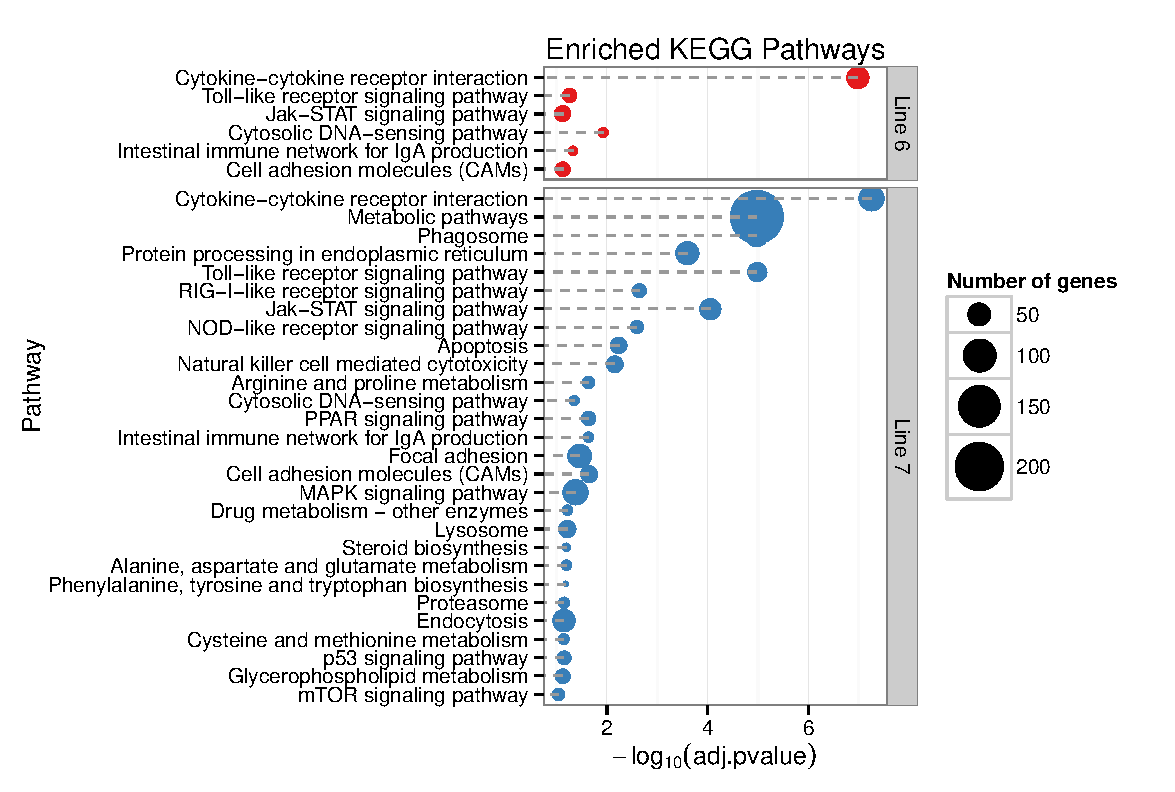
\includegraphics[width=7in]{line67_KEGG_cleveland.pdf}
\end{center}
\caption{
{\bf Enriched KEGG pathways.} Rest of figure 2  caption.  Caption 
should be left justified, as specified by the options to the caption 
package.
}
\label{line67_kegg}
\end{figure}

\begin{figure}[!ht]
\begin{center}
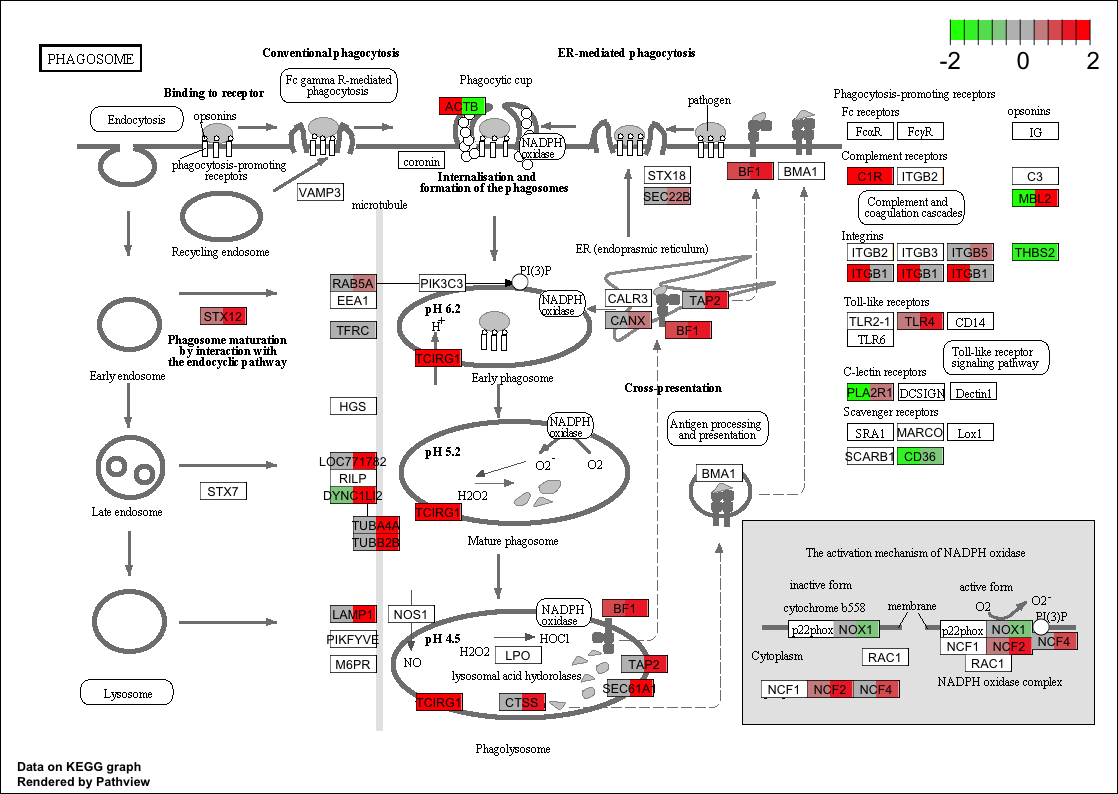
\includegraphics[width=6in]{gga04145_degenes_multi.png}
\end{center}
\caption{
{\bf Enriched KEGG pathways in line 7.}  Rest of figure 2  caption.  Caption 
should be left justified, as specified by the options to the caption 
package.
}
\label{kegg_phagosome}
\end{figure}

\begin{figure}[!ht]
    \begin{center}
        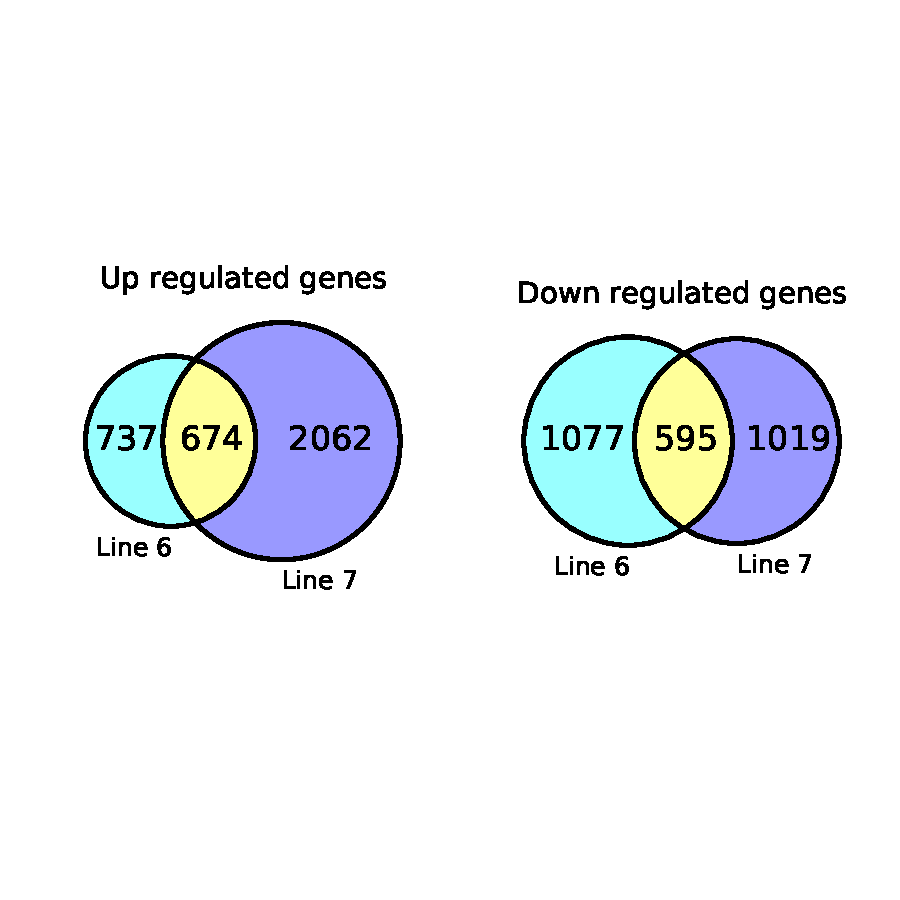
\includegraphics[width=6in]{degenes_venn.pdf}
    \end{center}
    \caption{
        {\bf Differential-expressed genes in response to MDV infection}
    }
    \label{degenes_venn}
\end{figure}

\section*{Tables}

\begin{table}[!ht]
\caption{
\bf{Gene models summary}}
\begin{tabular}{ccc}
\hline
Method & Gene & Isoform \\
\hline
Assembly & 25,290 & 54,044 \\
Cufflinks & 21,345 & 36,218 \\
Combined & 24,980 & 46,613 \\
\hline
\end{tabular}
\begin{flushleft}Number of genes and isoforms from gene models
built from \textit{de novo} assembly and Cufflinks.
Combination of both methods decreased the number of genes
and isoforms by merging fragmented transcripts to
form more complete gene models.
\end{flushleft}
\label{tab:gene_models}
\end{table}

\begin{table}[!ht]
\caption{
\bf{Genes regulated in opposite direction}}
\begin{tabular}{cccccc}
\hline
Gene & Entrez ID & Fold Change & \\
 & & Line 6 & line 7 \\
\hline
TAF1D & 419002 & +1.08 & -1.13 \\
LYG2 & 395708 & -1.70 & +2.57 \\
SFTPA1 & 395308 & -5.12 & +3.51 \\
LOC424145 & 424145 & +1.57 & -1.68 \\
LL & 423630 & -3.30 & +8.31 \\
SERPINB10 & 395715 & -1.12 & +0.87 \\
\hline
\end{tabular}
\begin{flushleft}
    (-) down-regulated, (+) up-regulated
\end{flushleft}
\label{tab:opposite}
\end{table}

\begin{table}[!ht]
\caption{
\bf{DEU between Line 6 and Line 7 in infected birds}}
\begin{tabular}{cccccccc}
\hline
& & & & Line 6 ($\Psi$) & & Line 7 ($\Psi$) & \\
Type & Event ID & Ensembl & Symbol  & Un & Inf & Un & Inf \\
\hline
SE & chr2:13729.ev2 & ENSGALG00000010973 & \textbf{TRA2A} & 0.45 & \textbf{0.75} & 0.58 & 0.50 \\
SE & chr5:634.ev3 & ENSG00000127152* & BCL11B & 0.07 & \textbf{0.31} & 0.06 & 0.04 \\
SE & chr5:22858.ev1 & ENSGALG00000011127 & BCL11B & 0.07 & \textbf{0.30} & 0.06 & 0.04 \\
SE & chr2:13065.ev1 & ENSGALG00000013137 & INO80C & 0.14 & \textbf{0.35} & 0.96 & 0.86 \\
SE & chr20:14995.ev1 & ENSG00000124193* & SRSF6 & 0.43 & \textbf{0.72} & 0.54 & 0.34 \\
A5SS & chr7:24049.ev1 & ENSGALG00000009824 & \textbf{C7H2ORF77} & 0.50 & \textbf{0.73} & 0.32 & 0.38 \\
A5SS & chr3:18098.ev1 & ENSGALG00000013821 & \textbf{GEMIN6} & 0.84 & \textbf{0.61} & 0.81 & 0.85 \\
A3SS & chr1:6450.ev1 & ENSGALG00000027665 & \textbf{SYNGR1} & 0.46 & \textbf{0.22} & 0.68 & 0.60 \\
A3SS & chr2:13270.ev1 & ENSGALG00000026498 & \textbf{Unknown} & 0.12 & \textbf{0.71} & 0.10 & 0.34 \\
A3SS & chr19:12399.ev1 & ENSGALG00000005685 & \textbf{KSR1} & 0.23 & \textbf{0.56} & 0.28 & 0.35 \\
A3SS & chr1:6437.ev1 & ENSGALG00000012050 & \textbf{TNRC6B} & 0.57 & \textbf{0.39} & 0.95 & 0.93 \\
A3SS & chr18:11800.ev1 & ENSGALG00000002859 & \textbf{RAC3} & 0.31 & \textbf{0.15} & 0.33 & 0.39 \\
\hline
SE & chr17:11370.ev2 & ENSGALG00000004971 & URM1 & \textbf{0.07} & \textbf{0.03} & 0.18 & 0.23 \\
SE & chr2:12495.ev3 & ENSGALG00000005582 & \textbf{KLHL18} & \textbf{0.44} & \textbf{0.27} & 0.56 & 0.52 \\
SE & chr7:24327.ev1 & ENSGALG00000007511 & \textbf{ITGB2} & \textbf{0.17} & \textbf{0.22} & 0.02 & 0.01 \\
SE & chr2:12984.ev1 & ENSGALG00000012809 & ECI2 & \textbf{0.15} & \textbf{0.29} & 0.58 & 0.49 \\
SE & chr8:25247.ev1 & ENSGALG00000028790 & DNASE2B & \textbf{0.38} & \textbf{0.50} & 0.29 & 0.26 \\
SE & chr1:4653.ev1 & ENSGALG00000011682 & CNOT4 & \textbf{0.57} & \textbf{0.63} & 0.40 & 0.40 \\
SE & chr20:14907.ev3 & ENSGALG00000006522 & \textbf{HCK} & \textbf{0.46} & \textbf{0.59} & 0.99 & 0.97 \\
SE & chr4:21539.ev1 & ENSGALG00000015709 & \textbf{TACC3} & \textbf{0.87} & \textbf{0.94} & 0.76 & 0.72 \\
SE & chr2:32201.ev1 & ENSGALG00000012258 & GOLGA4 & \textbf{0.33} & \textbf{0.34} & 0.51 & 0.61 \\
SE & chr3:19470.ev1 & ENSGALG00000019979 & DYNLT1 & \textbf{0.23} & \textbf{0.22} & 0.02 & 0.02 \\
SE & chr19:12391.ev1 & ENSGALG00000005522 & \textbf{DYNLL2} & \textbf{0.01} & \textbf{0.02} & 0.19 & 0.25 \\
A5SS & chr6:23812.ev1 & ENSG00000107651* & \textbf{SEC23IP} & \textbf{0.02} & \textbf{0.12} & 0.50 & 0.43 \\
A5SS & chr2:12775.ev1 & ENSGALG00000011488 & \textbf{CMTM7} & \textbf{0.55} & \textbf{0.67} & 0.37 & 0.41 \\
A3SS & chr8:25257.ev1 & ENSGALG00000008939 & \textbf{FUBP1} & \textbf{0.58} & \textbf{0.74} & 0.41 & 0.46 \\
A3SS & chr9:25750.ev1 & ENSGALG00000010410 & \textbf{PFN2} & \textbf{0.71} & \textbf{0.78} & 0.53 & 0.50 \\
A3SS & chr4:21230.ev1 & ENSGALG00000011476 & \textbf{SEPT11} & \textbf{0.22} & \textbf{0.14} & 0.40 & 0.42 \\
A3SS & chr4:20185.ev1 & ENSGALG00000008507 & THOC2 & \textbf{0.48} & \textbf{0.47} & 0.31 & 0.22 \\
A3SS & chr11:8703.ev1 & ENSGALG00000020987 & \textbf{ZDHHC7} & \textbf{0.42} & \textbf{0.23} & 0.57 & 0.55 \\
A3SS & chr4:21136.ev1 & ENSGALG00000027908 & \textbf{LOC42228} & \textbf{0.72} & \textbf{0.61} & 0.87 & 0.91 \\
\hline
SE & chr12:8987.ev1 & ENSGALG00000008320 & EDEM1 & 0.96 & 0.99 & 0.91 & \textbf{0.72} \\
SE & chr4:20411.ev1 & ENSGALG00000023199 & HNRPDL & 0.39 & 0.40 & 0.30 & \textbf{0.18} \\
SE & chrZ:26257.ev1 & ENSGALG00000001745 & PSTPIP2 & 0.06 & 0.04 & 0.13 & \textbf{0.26} \\
SE & chr1:6316.ev3 & ENSG00000058272* & PPP1R12A & 0.99 & 0.97 & 0.96 & \textbf{0.77} \\
SE & chr1:4478.ev2 & ENSGALG00000009029 & TSPAN12 & 0.09 & 0.15 & 0.20 & \textbf{0.46} \\
SE & chr4:20075.ev1 & ENSGALG00000006157 & DDX26B & 0.67 & 0.61 & 0.58 & \textbf{0.84} \\
SE & chr6:23515.ev1 & ENSGALG00000003861 & HERC4 & 0.31 & 0.37 & 0.45 & \textbf{0.06} \\
SE & chr26:16840.ev1 & ENSGALG00000000533 & SRSF3 & 0.36 & 0.38 & 0.30 & \textbf{0.16} \\
SE & chr11:8507.ev2 & ENSGALG00000000904 & \textbf{C11H16ORF57} & 0.91 & 0.98 & 0.84 & \textbf{0.78} \\
SE & chr1:4323.ev1 & ENSGALG00000006409 & PODXL & 0.21 & 0.34 & 0.26 & \textbf{0.13} \\
SE & chrZ:26582.ev2 & ENSGALG00000014642 & LOC374195 & 0.60 & 0.57 & 0.70 & \textbf{0.81} \\
SE & chr6:23833.ev1 & ENSG00000175029* & CTBP2 & 0.38 & 0.38 & 0.23 & \textbf{0.12} \\
A5SS & chr15:10720.ev1 & ENSGALG00000002487 & \textbf{SFSWAP} & 0.58 & 0.73 & 0.55 & \textbf{0.41} \\
A5SS & chr7:24350.ev1 & ENSGALG00000008038 & \textbf{SF3B1} & 0.41 & 0.57 & 0.55 & \textbf{0.31} \\
A3SS & chr2:13147.ev1 & ENSGALG00000014915 & \textbf{THOC1} & 0.33 & 0.48 & 0.33 & \textbf{0.23} \\
A3SS & chr23:15908.ev1 & ENSGALG00000000720 & LOC419563 & 0.12 & 0.06 & 0.17 & \textbf{0.30} \\
A3SS & chr8:25157.ev1 & ENSGALG00000005162 & RNPC3 & 0.45 & 0.64 & 0.58 & \textbf{0.33} \\
A3SS & chrZ:27197.ev1 & ENSGALG00000000189 & \textbf{YTHDC2} & 0.44 & 0.59 & 0.42 & \textbf{0.32} \\
A3SS & chr23:15983.ev1 & ENSG00000163875* & \textbf{MEAF6} & 0.28 & 0.57 & 0.40 & \textbf{0.29} \\
A3SS & chr5:21970.ev1 & ENSGALG00000009421 & \textbf{SRSF5} & 0.55 & 0.72 & 0.54 & \textbf{0.39} \\
\hline
SE & chr27:17351.ev1 & ENSGALG00000001107 & GOSR2 & 0.73 & 0.92 & 0.38 & 0.60 \\
\hline
\end{tabular}
\begin{flushleft}
    *human homologs, Un=uninfected, Inf=infected
\end{flushleft}
\label{tab:line67i_diff_line67u}
\end{table}

\begin{table}[!ht]
\caption{
\bf{DEU Genes in Spliceosome pathway}}
\begin{tabular}{cccccc}
\hline
Gene ID &  Ensembl & Symbol  & $-log2$FC* & \\
        & & & Line 6 & Line 7 \\
\hline
chr26:16840 & ENSGALG00000000533 & SRSF3 & 0.43 & 0.18 \\
chr2:13147 & ENSGALG00000014915 & THOC1 & -- & 0.21 \\
chr5:21970 & ENSGALG00000009421 & SRSF5 & -- & 0.18 \\
chr2:13729 & ENSGALG00000010973 & TRA2A & -- & -- \\
chr4:20185 & ENSGALG00000008507 & THOC2 & -- & -- \\
chr7:24350 & ENSGALG00000008038 & SF3B1 & -- & -- \\
\hline
\end{tabular}
\begin{flushleft}
    * FDR $<$ 0.05
\end{flushleft}
\label{tab:spliceosome}
\end{table}

\begin{table}[!ht]
\caption{
\bf{Pathways containing \textit{RAC3, ITGB2, PFN2} and \textit{PPP1R12A}}}
\begin{tabular}{ccc}
\hline
Pathway ID &  Description & Gene \\
\hline
hsa04810 & Regulation of actin cytoskeleton & \textit{RAC3, ITGB2, PPP1R12A, PFN2} \\
hsa04015 & RAP1 signaling pathway & \textit{RAC3, ITGB2, PFN2} \\
hsa04650 & Natural killer cells cytotoxicity & \textit{RAC3, ITGB2} \\
hsa05416 & Viral myocarditis & \textit{RAC3, ITGB2} \\
hsa04510 & Focal adhesion & \textit{RAC3, PPP1R12A} \\
\hline
\end{tabular}
\begin{flushleft}
\end{flushleft}
\label{tab:integrin}
\end{table}

\begin{table}[!ht]
\caption{
\bf{SNPs in exons}}
\begin{tabular}{ccccccc}
\hline
Gene &  Chromosome & Position & Reference & Alternative & & Strand \\
&  & & & Line 6 & Line 7 \\
\hline
ITGB2 & 7 & 7183696 & C & \textit{T} & C & - \\
PFN2 & 9 & 23221934 & -  - & & \textit{AA} & + \\
\hline
\end{tabular}
\begin{flushleft}
\end{flushleft}
\label{tab:spliceosome}
\end{table}

\begin{table}[!ht]
\caption{
\bf{Results from human splicing finder}}
\begin{tabular}{|l|p{1cm}|p{3cm}|l|l|l|l|}
\hline
Gene &  cDNA Position & Linked SR protein & Type & Reference Motif & Mutant Motif & Variation \\
\hline
PFN2 & 2068 & Tra2-$\beta$ & ESE & AAAAT (81.02) & AAAAa & +16.19\% \\
 & 2069 & Tra2-$\beta$ & ESE & & AAAaa (94.14) & New site \\
 & 2070 & Tra2-$\beta$ & ESE & & AAAaaT (81.02) & New site \\
 & 2066 & & ESS$^{2}$ & & ACAAAAaa (38.13) & New site \\
 & 2067 & & ESS$^{2}$ & & CAAAAaaT (28.85) & New site \\
\hline
ITGB2 & 20 & SC35 & ESE$^{1}$ & TGCTCATG (78.19) & & Site broken \\
 & 22 & SF2/ASF(IgM-BRCA1) & ESE$^{1}$ & CTCATGG (77.23) & CTCACGG (91.15) & +18.03\% \\
 & 22 & SF2/ASF(IgM-BRCA1), SF2/ASF & ESE$^{1}$ & CTCATGG (77.23) & CTCACGG (89.23) & +15.53\% \\
 & 22 & SF2/ASF, SF2/ASF(IgM-BRCA1) & ESE$^{1}$ & CTCATGG (74.55) & CTCACGG (91.15) & +22.27\% \\
 & 22 & SF2/ASF, SF2/ASF & ESE$^{1}$ & CTCATGG (74.55) & CTCACGG (89.23) & +19.69\% \\
 & 24 & SRp55 & ESE$^{1}$ & & CACGGA (79.30) & New site \\
 & 26 & SF2/ASF(IgM-BRCA1) & ESE$^{1}$ & & CGGAGAT (80.00) & New site \\
 & 26 & SF2/ASF & ESE$^{1}$ & & CGGAGAT (75.36) & New site \\
 & 21 & & ESS$^{3}$ & & GCTCACGG (63.35) & New site (-5.59) \\
 & 23 & & ESS$^{3}$ & TCATGGAG (61.41) & & Site broken (3.16) \\
 & 23 & & ESS$^{3}$ & ATGGAGAT (64.83) & ACGGAGAT & -5.16\% \\
 & 24 & & ESS$^{4}$ & CATGGA (65.48) & CACGGA (65.48) & 0\% \\
\hline

\end{tabular}
\begin{flushleft}
    $^{1}$ESE Finder matrices for SRp40, SC35, SF2/ASF and SRp55 proteins.
    $^{2}$Predicted PESS Octamers from Zhang \& Chasin.
    $^{3}$Silencer motif from Sironi et al.
    $^{4}$hnRNP motif.
\end{flushleft}
\label{tab:spliceosome}
\end{table}

\end{document}
